Data integration addresses to integrate existing databases. Synonyms for data integration are information fusion, data consolidation, data cleansing or data warehousing. The goal of data integration is almost always to simplify the access to a range of existing information systems through a central, integrated component with a unified interface for users and applications. Therefore, integrated information systems provide a unified view on the data sources. Existing information systems can be diverse: Classical relational database systems, files, data accessed by web services or HTML formulas, data generating applications or even other integrated information systems. (from \cite[p. 3-4]{DBLP:books/dp/LeserN2006}, own translation).\\
Today, data is classified into three diverse categories. Structured data like it is stored in relational databases, have a predefined structure through a schema.
Semi-structured data also have a schema, but they can deviate from the schema. An example of semi-structured data is a XML file without an accompanying XML schema. The third class is unstructured data and contains, as the name implies, no given structure. Typical unstructured data is natural language text.
(from \cite[p. 17]{DBLP:books/dp/LeserN2006}, own translation).\\
If we speak of diverse information systems we usually mean heterogeneous systems. Heterogeneity exists among data sources as well as between data sources and the integrated system. In most of all integrated information systems only the latter heterogeneity matters, as data sources often do not communicate among themselves. 
To bridge heterogeneity, it is obviously necessary to translate queries and to implement missing functionality in the integrated system. Table \ref{kinds-of-heterogeneity} shows an overview of existing kinds of heterogeneity (from \cite[p. 60/61]{DBLP:books/dp/LeserN2006}, own translation).

\begin{table}[]
\centering
\begin{tabular}{|l|p{0.7\textwidth}|}
\hline
 \textbf{Technical  heterogeneity}  &  includes all problems to realize the access of the data of the data sources technically. This heterogeneity is overcome if the integrated system is able to send a query to a data source and that data source principally understands the query and produces a set of data as result.\\ \hline
 \textbf{Syntactic  heterogeneity}    &  includes problems in the illustration of information. This heterogeneity is overcome if all information meaning the same are illustrated equally.\\ \hline
 \textbf{Data model  heterogeneity} &  means problems in the presentation of data of the used data models. This heterogeneity is solved if the data sources and the integrated system use the same data model.\\ \hline
 \textbf{Structural  heterogeneity}    &  includes differences in the structural representation of information. This heterogeneity is solved if semantic identical concepts are also structural equally modeled. \\ \hline
 \textbf{Schematic  heterogeneity} &  Important special case of the structural heterogeneity, whereby there are differences in the used data model.\\ \hline
 \textbf{Semantic  heterogeneity}    &  Includes problems regarding the meaning of used terms and concepts. This heterogeneity is solved if the integrated system and the data source really mean the same by the used names for schema elements. Equal names means consequently equal meaning.\\ \hline
\end{tabular}
\caption{Kinds of heterogeneity (from \cite[p. 60/61]{DBLP:books/dp/LeserN2006}, own translation)}
\label{kinds-of-heterogeneity}
\end{table}

In general, there are two different types of data integration: The materialized integration and the virtual integration. The difference between these two approaches is as follows: At materialized integration the data to be integrated is stored  into the integrated system itself, so on a central point. The data in the data sources remains but for querying the materialized view is used. At virtual integration, the data is only transported from the data source to the integrated system while the query processing. This temporary data is then again discarded. So integration isn't done once but on each query. Of course, an integrated information system can use both principles. Such a system is called hybrid. Both types have in common that a query is processed on a global schema. For the virtual integrated system, the data only exists virtual, thus relations between data sources and the global schema have to be specified and on query time the query has to be split into into query schedules. The schedules are responsible to extract the needed information from the different data sources and subsequently merge and transform the data (from \cite[p. 86-88]{DBLP:books/dp/LeserN2006}, own translation).

\section{Heterogeneity}
Information systems providing not the same methods, models and structures for accessing their data are called \textit{heterogeneous}. It is often the case, that distributed systems (and therefore are maintained independently) tend to be heterogeneous. In other words, distribution leads often to heterogeneity but not necessarily. De facto, it is to observe, that data sources tend to be the more heterogeneous the more they are autonomous. Two independent systems will in practice always  be heterogeneous, even if they contain the same kind of data. Heterogeneity arises from different requirements, different developers and different temporal developments. It even occurs if initially identical software systems are used but over time they were adapted to the specific enterprise's needs. This process is called \textit{customizing}. 

As the understanding of heterogeneity is essential for further proceeding, we will go a little more in depth for each kind of heterogeneity:
\begin{itemize}
\item Technical  heterogeneity
\item Syntactic  heterogeneity
\item Data model heterogeneity
\item Structural  heterogeneity
\item Schematic  heterogeneity
\item Semantic  heterogeneity
\end{itemize}

\section{Distribution}
\textcolor{red}{From: \cite[chapter 3.1 (p.51-54)]{DBLP:books/dp/LeserN2006}}

An issue of data integration is the distribution of data to be integrated. We speak thereby of data which lies on different systems. It should be noted that it is assumed that the access to the data is ensured, i.d. the systems are connected. A common example of distribution are data sources which can be accessed by a web interface using a browser: The Browser shows only a snippet of the data provided by a web server. The data itself is managed by the web server or one of the headed data sources. 
Data distribution isn't plainly an annoyance as it is often an intended design decision. Data distribution is handy for load balancing, reliability and protection against data loss. Thereby is the distribution controlled on a central point. The consistency of data is assured using sophisticated mechanisms like the 2-phase.commit protocol. Contrary, in a typical data integration project, distribution of data has historical evolved or is conditioned organizational and is thus uncontrolled redundant.

Distribution can be structured into logical and physical distribution. Data is \textit{physical} distributed, if it lies onto physical different systems which can also geographically be located on different places. In turn, data is \textit{logical} distributed, if there exists multiple possible locations for storing a datum. 

\subsection{Physical distribution}
To integrate physical distributed data there have to be overcome several issues: The first step is to detect the physical storage location of the data. Therefore computer, server and port and network have to be identifiable and locatable. For identification, applications used in the internet use Uniform Resource Locators (URLs) to identify remote computers and services not knowing there exact location. The part of locating is the responsibility of the network layer of the computers, using protocols like TCP/IP.

The second problem resulting from physical distribution is data stored in different schemas. Common query languages don't provide the possibility to query tables using different schemas. There are two possible ways to overcome this hurdle:
\begin{itemize}
\item Separating a query into several schema specific queries and consolidating the results in the integrated system.
\item Developing a language able to handle several schemas in a posed query.
\end{itemize}

The third problem are changed requirements for the query optimizer: In a central database the optimizer's key function is minimizing  the accesses to the secondary storage whereas for a distributed database the accesses over the network should be held as small as possible for this kind of accesses needs considerably more time than accesses to the secondary storage.  

\subsection{Logical distribution}
If identical data is located on different places inside the system, we speak of a logical distribution. The key property of logical distribution is therefore the \textit{overlapping of the intension} of different data storage locations. Thereby it is insignificant where these systems physically really are. Two database instances on one computer induce already distribution issues.

A central point here plays the redundancy in a system. A system is called redundant, if semantic equal data can be located at different places. In order to get a consistent view of a redundant system, redundancy has to be strictly controlled (e.g. using triggers or replication mechanisms). At anytime it has to be assured that the same data is at all different places. But data integration typical has to deal with \textit{uncontrolled redundancy} for each data source is maintained independently. This fact results to several problems:
\begin{itemize}
\item \textbf{Localization}: For a user it isn't obvious in which sources to find specific data. As a result, the integrated system has to provide meta data allowing \textit{to locate data}. This can e.g. done by a catalog of all schemas and their descriptions or a global schema with mappings to source schemas.
\item \textbf{Duplicates}: If it is possible that data exists on multiple locations, there will exist duplicates, i.d. objects stored on both locations. These objects have to be recognized by the integrated system.
\item \textbf{Inconsistencies}: Redundant data can contain inconsistencies, which have to be resolved for a homogeneous presentation.
\end{itemize}

\section{Architectures}

Integrated systems evolved from distributed databases which in turn are based on the classical monolithic database. In the following basic database concepts, on which integrated systems base, are explained. Additionally different types of integrated systems are presented shortly.

The \textbf{monolithic database} is subdivided into three layers as seen in \ref{MonolithicDatabaseArchitecture}: The \textit{internal (or physical) view} is responsible for the storage of the data on the respective database. One layer upwards comes the \textit{conceptual (or logical) view} modeling the data on a conceptual way. The conceptual schema defines which data model is used, which data is stored in the DBMS and the relations among the data.
Splitting the data into the internal and conceptual view, makes the data independent from the physical storage medium. The top layer is called \textit{external (or export) view} and is being concerned with modeling of data as well as the conceptual view. However it isn't modeled the whole application domain. The external view only specifies which part of the conceptual schema is provided to the respective application. An export schema is initially a subset of the conceptual schema, but can be transformed and aggregated. In the external view are defined access restrictions, too. Splitting up conceptual and external view ensures \textit{logical data independence} (\cite[p. 84/85]{DBLP:books/dp/LeserN2006}, own translation).
\begin{figure}[H]
	\begin{center}
		\includegraphics[scale=0.5]{figures/monolithicalDatabaseArchitecture.pdf}
	\end{center}
	\caption{Architecture of a monolithic database \textcolor{red}{TODO: own figure but inspired by book; cite properly}}
	\label{MonolithicDatabaseArchitecture}
\end{figure}
Next comes the \textbf{distributed database} architectures as shown in \ref{DistributedDatabaseArchitecture}. The idea is to distribute the data onto several systems (physical and logical), but a user should be able to query all data at once. In order to achieve this, the architecture is subdivided into \textit{four layers}. Each data source owns a local internal and local conceptual schema. The latter only mirrors the data managed by the local database. Dependent on the used distribution strategy, the local conceptual schema is equal to the global conceptual schema  or an extract from it. Common distribution strategies are vertical and horizontal partitioning: 
\begin{itemize}
\item horizontal partitioning: Data of big tables is distributed per tuples on different computers. A union operation consolidates these parts again.
\item vertical partitioning: Data of big tables is distributed per attributes on different computers. Each partition contains additionally a shared key attribute. This makes it possible to consolidate the partitions with a join operation.
\end{itemize}
On top of the local conceptual schemes stands a global conceptual schema. This schema models the whole application domain and is the central point of reference for the external schemes playing the same role as in the three-layers-architecture.
Distributed databases are close coupled. They are strictly checked while conception and operation and thus the main problems of heterogeneity (like structural and semantic heterogeneity) don't occur (\cite[p. 91-93]{DBLP:books/dp/LeserN2006}, own translation).
\begin{figure}[H]
	\begin{center}
		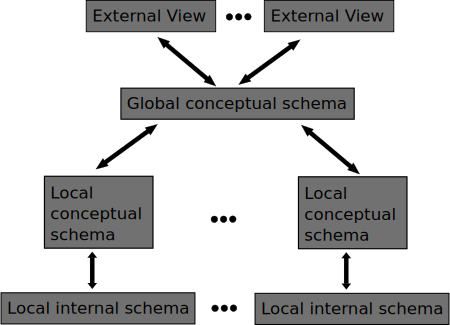
\includegraphics[scale=0.5]{figures/distributedDatabaseArchitecture.pdf}
	\end{center}
	\caption{Architecture of a distributed database}
	\label{DistributedDatabaseArchitecture}
\end{figure}
For allowing to connect heterogeneous databases, \textbf{Multidatabase Systems} (MBS) have been evolved (shown in \ref{MBSDatabaseArchitecture}). MBS are collections of autonomous databases being loosely linked. Each database grants external applications access to its data. The access is done using a database language which allows to query several databases in one query. Such a language is called multidatabase language. To obtain the autonomy  of the involved databases, a MBS has no global conceptual schema. Instead, each local database keeps an export schema defining which part of the local conceptual schema is provided to external applications.  
It is assumed that no data model heterogeneity is contained in a MBS, i.d. all databases use the same data model or either the multidatabase language or the local data source provide a translation to the global data model. Now, each application can create its own external schema, which integrates one or more data sources. So its the task of the application doing the integration task. A MBS provides only a suitable language for querying (\cite[p. 93/94]{DBLP:books/dp/LeserN2006}, own translation).	
\begin{figure}[H]
	\begin{center}
		\includegraphics[scale=0.5]{figures/MultidatabaseArchitecture.pdf}
	\end{center}
	\caption{Architecture of a  multidatabase system}
	\label{MBSDatabaseArchitecture}
\end{figure}
In contrast to MBS, \textbf{federated database management systems} (FDBMS) have a global conceptual schema as seen in \ref{FDBMSArchitecture}. This schema is the central and stable point of reference for all external schemes and there applications. But in contrast to distributed databases the global schema results after the local schemes with the goal to provide an integrated view of existing and heterogeneous data sets. Data sources keep a high degree of autonomy.
The used data model in the global scheme is known as canonical data model. Every local export schema has to be mapped to this global schema. Thus, in order to support heterogeneity in the data model, another layer is needed between local conceptual schema and the local export schema. This new layer is called \textit{local component schema} and translates the local conceptual schema into the canonical data model. The translation is done by a software component called \textit{Wrapper}. All in all, a FDBMS consists of five different layers.
The global schema can be created either by schema integration or schema mapping. Both variants are introduced later \textcolor{red}{(TODO)}
(\cite[p. 94/95]{DBLP:books/dp/LeserN2006}, own translation).\\
\begin{figure}[H]
	\begin{center}
		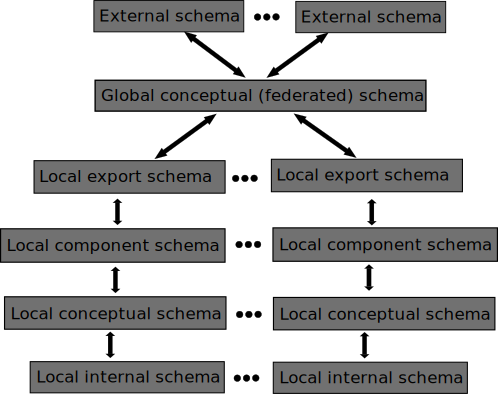
\includegraphics[scale=0.5]{figures/federatedDatabaseArchitecture.pdf}
	\end{center}
	\caption{Architecture of a  federated database management systems (FDBMS)}
	\label{FDBMSArchitecture}
\end{figure}

\textbf{Mediator-based information systems} (as seen in \ref{MediatorBasedArchitecture}) are a generalization of the previous architectures, as they know only two separate components, namely Wrappers and Mediators: Wrappers are software components responsible for the access to a solely data source. A Wrapper has to break down technical, data model, schematic and interface heterogeneity. Mediators access one or more wrappers and deliver a specific value, normally structural and semantic data integration.
In this architecture, data sources usually don't know of the existence of the integrated system, and so autonomy is preserved for all data sources (\cite[p. 97]{DBLP:books/dp/LeserN2006}, own translation).
\begin{figure}[H]
	\begin{center}
		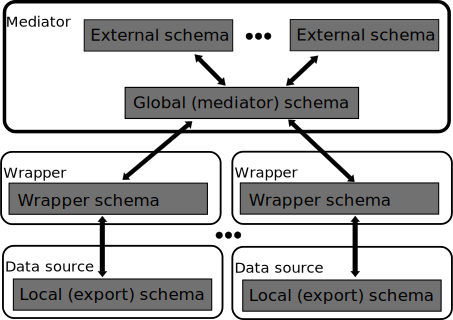
\includegraphics[scale=0.5]{figures/MediatorBasedArchitecture.pdf}
	\end{center}
	\caption{Architecture of a  mediator-based information system}
	\label{MediatorBasedArchitecture}
\end{figure}
In \textbf{peer data management systems} (PDMS) there is no separation between data source and integration system. Query can be posed from every system to every other system within the integrated system. The other system than tries to calculate responses with own or other sourced data. So each participant of the integrated system, a so-called peer, is a mediator and a data source at the same time.  

\textbf{Ontology-based integration} is an approach of semantic integration using ontologies. This approach assumes that the discourse range is able to be specified so exact, that semantic heterogeneity can be solved in a formal model by logical inference. Hereby, the formal model is called ontology. Ontologies define the vocabulary describing all concepts of the field of application, and the relations between these concepts. At the same time, an ontology often serves as global schema of the integration layer. For specifying ontologies, special classes of logics are used, the so-called description logics. With description logics, classes of a domain and relations among them can be specified much more precise than with the relational data model. (\cite[p. 267]{DBLP:books/dp/LeserN2006}, own translation).\\